\chapter{Marco teórico}
\label{chap:marco-teorico}

% Versión 1 del capítulo 2 (2026-10-04). Hilo narrativo adaptado de las secciones
% 5.1 a 5.6 del plan de trabajo aprobado. Notación idéntica a la del capítulo 3.

Este capítulo reúne los fundamentos sobre los que se construyó el trabajo y los presenta como una secuencia en la que cada sección plantea la pregunta que responde la siguiente. Parte de la física de los muones cósmicos y de su paso por la roca, que explica por qué pueden usarse como sonda de densidad. Describe después cómo se forma una imagen muográfica por transmisión y qué información contiene y cuál no, y muestra que su calidad está gobernada por la estadística de conteo. Introduce a continuación los modelos de aprendizaje profundo que se han empleado para mejorar imágenes de baja estadística, revisa su aplicación en muografía, discute el papel de los datos sintéticos en su entrenamiento y termina con las métricas con las que se juzga la calidad de una imagen. Los procedimientos concretos con los que estos conceptos se aplicaron se describen en el \cref{chap:metodologia}.

% =============================================================================
\section{Muones cósmicos como sonda natural}
\label{sec:mt-muones}

La Tierra recibe de forma continua rayos cósmicos primarios, en su mayoría protones y núcleos de helio, que interactúan con los núcleos de la alta atmósfera y producen cascadas de partículas secundarias. Entre ellas abundan los piones y kaones cargados, cuya desintegración da lugar a los muones. Los muones se producen típicamente a unos 15~km de altura y, aunque su vida media en reposo es de solo 2,2~$\mu$s, la dilatación relativista del tiempo permite que una fracción importante de ellos alcance la superficie \parencite{gaisser2016,pdg2022}. El muon tiene la misma carga que el electrón y una masa unas doscientas veces mayor, de 105,7~MeV/$c^{2}$; no participa en la interacción fuerte y, por su masa, pierde energía por radiación mucho más lentamente que el electrón. Esas propiedades explican que, con energías del orden de los GeV o mayores, pueda atravesar cientos de metros e incluso kilómetros de roca.

El flujo de muones en la superficie se describe por su intensidad diferencial $\Phi(E,\zeta)$, el número de muones por unidad de área, de tiempo, de ángulo sólido y de energía, que depende de la energía $E$ y del ángulo cenital $\zeta$ de la dirección de llegada. A nivel del mar, la intensidad integral de los muones verticales con momento superior a 1~GeV/$c$ es de unos 70~m$^{-2}$\,s$^{-1}$\,sr$^{-1}$, lo que equivale aproximadamente a un muon por centímetro cuadrado y por minuto sobre un detector horizontal, y la energía media de los muones es de unos 4~GeV \parencite{pdg2022}. El espectro es casi plano por debajo de 1~GeV, se vuelve más pronunciado entre 10 y 100~GeV, donde reproduce la pendiente del espectro primario, cercana a $E^{-2{,}7}$, y decae aún más rápido a energías mayores, porque los piones más energéticos tienden a interactuar en la atmósfera antes de desintegrarse. La distribución angular de los muones de unos 3~GeV es aproximadamente proporcional a $\cos^{2}\zeta$; a energías menores es más pronunciada y a energías muy altas se aplana, porque en las trayectorias inclinadas los piones recorren más atmósfera tenue y tienen más oportunidad de desintegrarse \parencite{pdg2022,gaisser2016}. Como los muones de baja energía de las trayectorias inclinadas se desintegran o se detienen antes de llegar al suelo, la energía media aumenta con el ángulo cenital, aunque el flujo total disminuye. La razón entre muones positivos y negativos es algo mayor que la unidad, como reflejo de la carga positiva de los primarios.

Para la muografía resulta central el flujo integral, que cuenta los muones con energía superior a un umbral $E_{\min}$ en una dirección dada:
\begin{equation}\label{eq:mt-flujo-integral}
\Phi_{\mathrm{int}}(E_{\min},\zeta) = \int_{E_{\min}}^{\infty}\Phi(E,\zeta)\,\mathrm{d}E ,
\end{equation}
donde $\Phi_{\mathrm{int}}$ se expresa en cm$^{-2}$\,s$^{-1}$\,sr$^{-1}$ cuando $\Phi$ se expresa en cm$^{-2}$\,s$^{-1}$\,sr$^{-1}$\,GeV$^{-1}$ y las energías en GeV. Como se muestra en la sección siguiente, el paso por la roca impone precisamente un umbral de energía, de modo que la \cref{eq:mt-flujo-integral} conecta el espectro de los muones con lo que registra un detector situado al pie de un volcán. Para evaluarla se emplean parametrizaciones ajustadas a las mediciones. La fórmula de Gaisser describe bien el flujo a energías altas y ángulos cenitales moderados, y \textcite{guan2015muonflux} la modificaron para extenderla a energías bajas y a todo el rango de ángulos cenitales, que es el régimen de las observaciones casi horizontales de la muografía volcánica \parencite{gaisser2016}.

% =============================================================================
\section{Pérdida de energía y alcance de los muones en la roca}
\label{sec:mt-interaccion}

Un muon que atraviesa la roca pierde energía de manera prácticamente continua. La pérdida media por unidad de espesor másico se describe con dos términos \parencite{groom2001,pdg2022}: uno de ionización, $a(E)$, que domina a energías bajas y varía muy lentamente con la energía, y uno radiativo, $b(E)\,E$, que agrupa la radiación de frenado, la producción de pares y las interacciones fotonucleares y crece en proporción a la energía. Si $X$ denota el espesor másico recorrido, en g\,cm$^{-2}$, la pérdida media es la de la \cref{eq:mt-perdida-dedx}, y la energía en la que ambos términos se igualan, llamada energía crítica del muon, es del orden de varios cientos de GeV en la roca estándar, un material de referencia con $Z=11$, $A=22$ y densidad de 2,65~g\,cm$^{-3}$ \parencite{groom2001}. El término de ionización, descrito por la fórmula de Bethe, tiene un mínimo amplio en $\beta\gamma\approx3$--$4$, el régimen de las partículas de ionización mínima, y por encima de él crece solo de forma logarítmica, por lo que en la muografía, cuyos muones son en su mayoría relativistas, puede tratarse como casi constante.

Si $a$ y $b$ se toman constantes, la integración de la pérdida media a lo largo del recorrido, en la aproximación de frenado continuo, da la energía mínima que un muon necesita para atravesar un espesor másico $X$:
\begin{subequations}\label{eq:mt-perdida}
\begin{align}
-\frac{\mathrm{d}E}{\mathrm{d}X} &= a(E) + b(E)\,E, \label{eq:mt-perdida-dedx}\\
E_{\min}(X) &= \frac{a}{b}\left(\mathrm{e}^{bX}-1\right), \label{eq:mt-perdida-emin}
\end{align}
\end{subequations}
donde $a$ se expresa en GeV\,cm$^{2}$\,g$^{-1}$, $b$ en cm$^{2}$\,g$^{-1}$ y $E_{\min}$ en GeV. Para espesores pequeños, $bX\ll1$ y la \cref{eq:mt-perdida-emin} se reduce a $E_{\min}\approx aX$, el régimen dominado por la ionización; para espesores grandes, la energía mínima crece exponencialmente. En la roca estándar, con $a\approx2\times10^{-3}$~GeV\,cm$^{2}$\,g$^{-1}$ y $b\approx4\times10^{-6}$~cm$^{2}$\,g$^{-1}$, atravesar un kilómetro de roca, unos $2{,}65\times10^{5}$~g\,cm$^{-2}$, exige del orden de 1~TeV, una energía que solo alcanza una fracción muy pequeña de los muones del flujo \parencite{galgoczi2024}. La relación entre el espesor y la energía mínima, junto con la caída del espectro, es la que convierte la atenuación del flujo en una medida de la cantidad de materia atravesada.

La pérdida de energía no es el único efecto del paso por la roca. Las múltiples desviaciones de pequeño ángulo que el muon sufre en el campo eléctrico de los núcleos, conocidas como dispersión múltiple de Coulomb, cambian su dirección de forma aleatoria. La distribución del ángulo de desviación proyectado es aproximadamente gaussiana en su parte central, con una anchura que la fórmula de Highland, refinada por \textcite{lynch1991}, expresa como
\begin{equation}\label{eq:mt-dispersion}
\theta_{0} = \frac{13{,}6~\mathrm{MeV}}{\beta c p}\,z\,\sqrt{\frac{x}{X_{0}}}\left[1+0{,}038\,\ln\!\left(\frac{x\,z^{2}}{X_{0}\,\beta^{2}}\right)\right],
\end{equation}
donde $p$ es el momento, $\beta c$ la velocidad y $z$ la carga de la partícula, en unidades de la carga elemental, $x$ el espesor atravesado y $X_{0}$ la longitud de radiación del material, ambos en g\,cm$^{-2}$, y $\theta_{0}$ resulta en radianes \parencite{pdg2022}. La desviación es inversamente proporcional al momento, de modo que afecta sobre todo a los muones de baja energía. En una imagen muográfica, esos muones son precisamente los que cruzan los espesores pequeños de roca cerca del contorno del edificio, por lo que la dispersión múltiple desplaza su dirección de llegada respecto de la que tenían al entrar en la roca y difumina la transición entre la roca y el cielo. Por esa razón, el contorno de un volcán en una imagen muográfica no es un borde nítido, sino una franja en la que se mezclan direcciones.

% =============================================================================
\section{Formación de la imagen muográfica por transmisión}
\label{sec:mt-imagen}

La muografía por transmisión mide cuántos muones llegan a un detector desde cada dirección después de atravesar el objeto de estudio. Una dirección de observación se describe por su acimut $\alpha$ y su elevación $e$ sobre la horizontal, y el ángulo cenital de la misma dirección cumple $\cos\zeta=\sin e$. A lo largo de esa dirección, el muon recorre un trayecto $L(\alpha,e)$ en el que encuentra roca de densidad variable. La magnitud que gobierna su atenuación es la opacidad, o espesor másico, definida como la integral de línea de la densidad a lo largo del trayecto \parencite{lesparre2010,tanaka2023muography}. Con ella, el número esperado de muones registrados en una celda angular y la transmisión, que compara ese número con el que se registraría en la misma dirección sin roca interpuesta, son los de la \cref{eq:mt-imagen}:
\begin{subequations}\label{eq:mt-imagen}
\begin{align}
X(\alpha,e) &= \int_{L(\alpha,e)}\rho(\mathbf{r})\,\mathrm{d}\ell, \label{eq:mt-opacidad}\\
\lambda(\alpha,e) &= A\,\Delta\Omega\,t\;\Phi_{\mathrm{int}}\!\left(E_{\min}\!\left(X(\alpha,e)\right),\zeta\right), \label{eq:mt-conteo}\\
T(\alpha,e) &= \frac{\lambda(\alpha,e)}{\lambda_{\mathrm{libre}}(\alpha,e)}, \label{eq:mt-transmision}\\
\bar\rho(\alpha,e) &= \frac{X(\alpha,e)}{L(\alpha,e)}. \label{eq:mt-densidad-media}
\end{align}
\end{subequations}
En la \cref{eq:mt-opacidad}, $\rho(\mathbf{r})$ es la densidad en el punto $\mathbf{r}$ del trayecto, en g\,cm$^{-3}$, y $\mathrm{d}\ell$ el elemento de longitud, en cm, de modo que $X$ resulta en g\,cm$^{-2}$. En la \cref{eq:mt-conteo}, $\lambda$ es el número esperado de muones, adimensional; $A$ es el área efectiva del detector, en cm$^{2}$; $\Delta\Omega$ el ángulo sólido de la celda, en sr, y $t$ el tiempo de exposición, en s. La expresión corresponde a un detector ideal; un instrumento real introduce, además, su aceptancia angular y su eficiencia \parencite{lesparre2010}. En la \cref{eq:mt-transmision}, $\lambda_{\mathrm{libre}}$ es el número esperado en la misma dirección cuando el muon solo atraviesa aire, y en la \cref{eq:mt-densidad-media}, $\bar\rho$ es la densidad media a lo largo del recorrido en la roca, de longitud $L$, en cm.

La \cref{eq:mt-imagen} contiene la propiedad que define el alcance de la técnica, que la \cref{fig:mt-proyeccion} ilustra. Cada dirección de observación es un píxel de la imagen, y el valor de ese píxel resume con un solo número toda la densidad encontrada a lo largo de un trayecto de cientos de metros. La imagen muográfica es, por lo tanto, una proyección del objeto sobre el espacio de direcciones y no una representación de su volumen: un conducto, una cavidad o un cuerpo denso modifican el conteo del píxel por el que pasan, pero la imagen no indica en qué punto del trayecto se encuentran.

\begin{figure}[htbp]
\centering
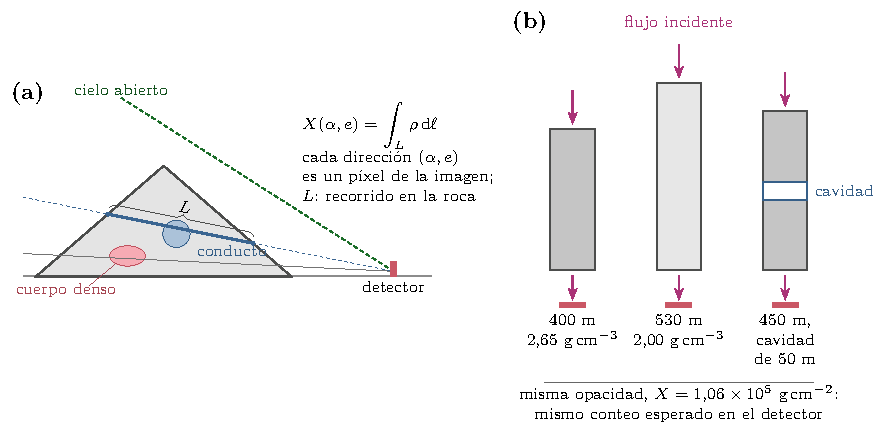
\includegraphics{fig2-1_opacidad_proyeccion.pdf}
\caption[La imagen muográfica por transmisión como proyección]{La imagen muográfica por transmisión como proyección (esquema sin escala). (a)~Cada dirección de observación $(\alpha,e)$ desde el detector define un trayecto; el píxel correspondiente registra la opacidad $X$ acumulada a lo largo del recorrido $L$ en la roca, incluidas las anomalías que encuentre, y la dirección de cielo abierto sirve de referencia para la transmisión. (b)~Ambigüedad entre espesor y densidad: 400~m de roca de 2,65~g\,cm$^{-3}$, 530~m de roca de 2,00~g\,cm$^{-3}$ y 450~m de roca de 2,65~g\,cm$^{-3}$ con una cavidad de 50~m tienen la misma opacidad, $1{,}06\times10^{5}$~g\,cm$^{-2}$, y producen el mismo conteo esperado. Fuente: elaboración propia.}
\label{fig:mt-proyeccion}
\end{figure}

Dos consecuencias se siguen de esa propiedad. La primera es que, para convertir la opacidad en una densidad, hace falta conocer la longitud del recorrido. La \cref{eq:mt-densidad-media} solo puede evaluarse si se conoce la superficie del terreno, normalmente mediante un modelo digital de elevación, y la posición del detector; sin esa información, la imagen no distingue entre una roca densa y una roca gruesa \parencite{lesparre2010,lechmann2021}. La segunda es que el problema inverso no tiene solución única. Como muestra el panel~(b) de la \cref{fig:mt-proyeccion}, distribuciones de densidad muy diferentes producen la misma opacidad y, por lo tanto, el mismo conteo esperado: una roca delgada y densa equivale a una gruesa y liviana, y una cavidad puede compensarse con un trayecto más largo. Por esta razón, la interpretación muográfica se apoya en contrastes. Se compara la opacidad o el conteo observado con el que produciría un modelo de referencia, por ejemplo el mismo edificio con densidad homogénea y topografía conocida, y se interpretan las desviaciones: un conducto de baja densidad produce un exceso de conteos respecto de su entorno y un cuerpo denso, un déficit.

Recuperar la distribución tridimensional de la densidad exige más información que la de una sola vista. Puede obtenerse combinando observaciones desde varias posiciones, en lo que constituye una tomografía muográfica, o mediante la inversión conjunta de los datos muográficos con otras mediciones, como las gravimétricas, que aportan sensibilidad a la masa en otras direcciones \parencite{nishiyama2022,lechmann2021,tanaka2023muography}. Con una sola vista, la muografía por transmisión entrega un mapa bidimensional de opacidad o de conteos, que es suficiente para localizar anomalías en el espacio de direcciones, pero no para situarlas en profundidad.

Las aplicaciones volcánicas de la técnica se han apoyado precisamente en esos mapas bidimensionales y en sus contrastes. Bajo el cráter del monte Asama se resolvió la estructura de densidad del fondo del cráter \parencite{tanaka2007asama}; en el Sakurajima, detectores gaseosos de trazas produjeron imágenes de alta definición y bajo ruido \parencite{olah2018sakurajima}, y en Colombia, el telescopio MuTe se diseñó para observar volcanes activos en zonas de difícil acceso, combinando paneles de centelleo con un detector Cherenkov de agua para filtrar el fondo \parencite{penarodriguez2020}. En todos los casos, la calidad de los contrastes obtenidos depende del número de muones registrados, que es el objeto de la sección siguiente.

% =============================================================================
\section{Estadística de conteo y tiempo de exposición}
\label{sec:mt-estadistica}

La llegada de muones a una celda angular del detector es una sucesión de eventos independientes y raros, que se modela como un proceso de Poisson. Si $\lambda$ es el número esperado de muones en la exposición $t$, de acuerdo con la \cref{eq:mt-conteo}, el conteo registrado $C$ sigue una distribución de Poisson, y de ella se derivan su valor esperado, su varianza y la relación entre la señal y el ruido:
\begin{subequations}\label{eq:mt-poisson}
\begin{align}
P(C=c) &= \frac{\lambda^{c}\,\mathrm{e}^{-\lambda}}{c!}, \qquad c=0,1,2,\dots, \label{eq:mt-poisson-pmf}\\
\mathrm{E}[C] &= \mathrm{Var}[C] = \lambda, \label{eq:mt-poisson-momentos}\\
\mathrm{SNR} &= \frac{\mathrm{E}[C]}{\sqrt{\mathrm{Var}[C]}} = \sqrt{\lambda}, \qquad \frac{\sqrt{\mathrm{Var}[C]}}{\mathrm{E}[C]} = \frac{1}{\sqrt{\lambda}}. \label{eq:mt-poisson-snr}
\end{align}
\end{subequations}
Todas las magnitudes de la \cref{eq:mt-poisson} son adimensionales. La señal, el número esperado de conteos, crece en proporción a la exposición; el ruido, medido por la desviación estándar, crece solo con su raíz cuadrada. En consecuencia, la relación señal-ruido es $\sqrt{\lambda}$ y el ruido relativo es $1/\sqrt{\lambda}$, como muestra la \cref{fig:mt-ruido}. Un píxel con un valor esperado de 100 conteos fluctúa típicamente un 10\,\%; uno con 10\,000 conteos, un 1\,\%. Para reducir el ruido relativo a la mitad hay que cuadruplicar la exposición, y reducir la exposición en un factor $k$ multiplica el ruido relativo por $\sqrt{k}$.

\begin{figure}[htbp]
\centering
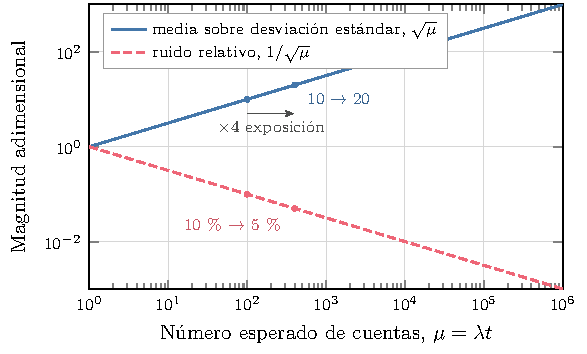
\includegraphics{fig2-2_ruido_conteo.pdf}
\caption[Relación señal-ruido y ruido relativo de un conteo de Poisson]{Relación señal-ruido, $\sqrt{\lambda}$, y ruido relativo, $1/\sqrt{\lambda}$, de un conteo de Poisson en función de su valor esperado $\lambda$, en escala logarítmica. Los puntos ilustran que cuadruplicar la exposición, de $\lambda=100$ a $\lambda=400$, duplica la relación señal-ruido y reduce el ruido relativo del 10 al 5\,\%. Curvas analíticas, sin datos del proyecto. Fuente: elaboración propia.}
\label{fig:mt-ruido}
\end{figure}

Esta dependencia determina el tiempo necesario para distinguir una anomalía. Si una anomalía cambia el número esperado de conteos de una región de $\lambda$ a $(1+\mathcal{C})\lambda$, donde $\mathcal{C}$ es el contraste relativo de la intensidad de conteo, el cambio solo se distingue de las fluctuaciones cuando supera algunas veces su desviación estándar. Si se exige que lo haga en $k$ desviaciones estándar, y se escribe $\lambda=r\,t$ con $r$ la tasa de conteo de la región, la condición y el tiempo de exposición que de ella resulta son
\begin{equation}\label{eq:mt-tiempo-deteccion}
|\mathcal{C}|\,\lambda \ge k\sqrt{\lambda}
\quad\Longleftrightarrow\quad
t \ge \frac{k^{2}}{\mathcal{C}^{2}\,r},
\end{equation}
donde $t$ y $1/r$ se expresan en la misma unidad de tiempo y $k$ y $\mathcal{C}$ son adimensionales. El tiempo necesario crece con el cuadrado del inverso del contraste: una anomalía con la mitad de contraste exige cuatro veces más exposición. Esta relación, de la misma naturaleza que el criterio de factibilidad formulado por \textcite{lesparre2010}, explica por qué las anomalías sutiles bajo grandes espesores de roca, donde la tasa $r$ es pequeña, exigen exposiciones de semanas o meses.

De lo anterior se sigue una precisión sobre el término \emph{alta estadística}. Una imagen de alta estadística no es una imagen sin azar, sino una con muchos conteos por píxel y, por lo tanto, con un ruido relativo pequeño, pero no nulo. Cuando una imagen de larga exposición se usa como referencia para juzgar otra, esa referencia conserva su propio ruido, y ninguna estimación puede coincidir exactamente con ella; la similitud alcanzable con una referencia finita tiene, por eso, un techo que depende de la estadística de la propia referencia.

El proceso de Poisson tiene, además, una propiedad que permite estudiar distintas exposiciones a partir de una sola medición o simulación. Si cada evento de un proceso de Poisson de media $\lambda$ se conserva de manera independiente con probabilidad $f$, los eventos conservados forman de nuevo un proceso de Poisson, de media $f\lambda$ \parencite{kingman1992}. En términos de conteos,
\begin{equation}\label{eq:mt-adelgazamiento}
C\sim\mathrm{Poisson}(\lambda), \quad C'\mid C\sim\mathrm{Bin}(C,f)
\quad\Longrightarrow\quad
C'\sim\mathrm{Poisson}(f\lambda), \qquad 0<f\le1,
\end{equation}
donde $C'$ es el conteo conservado y $f$ la fracción de conservación, ambos adimensionales. Como $f\lambda$ es el valor esperado que correspondería a una exposición $f\,t$, este adelgazamiento binomial produce, a partir de una imagen de exposición $t$, imágenes con la misma distribución que tendrían mediciones independientes de exposición $f\,t$. La equivalencia vale para cada imagen por separado: las imágenes reducidas que se obtienen de una misma imagen original comparten sus conteos y no son, entre sí, mediciones independientes.

% =============================================================================
\section{Aprendizaje profundo para la mejora de imágenes}
\label{sec:mt-aprendizaje}

La sección anterior mostró que el ruido de una imagen muográfica solo se reduce, por medios físicos, aumentando la exposición. La alternativa computacional consiste en estimar, a partir de la imagen ruidosa, la imagen que se habría obtenido con más exposición. Los filtros clásicos de suavizado reducen el ruido promediando píxeles vecinos, pero lo hacen a costa de la resolución espacial y difuminan precisamente los bordes y las anomalías pequeñas. El aprendizaje profundo aborda el problema de otro modo: aprende la relación entre imágenes degradadas y sus versiones de referencia a partir de ejemplos, y la aplica después a imágenes nuevas. Formalmente, dado un conjunto de pares formados por una entrada degradada $x$ y su referencia $y$, se ajustan los parámetros de una función $\hat y=G(x)$ para que su salida se aproxime a $y$ según una función de pérdida.

Las redes neuronales convolucionales son la arquitectura habitual para esta tarea. Cada capa aplica un conjunto de filtros que se aprenden durante el entrenamiento y que recorren la imagen con pesos compartidos, de modo que la red detecta un mismo patrón en cualquier posición y construye, capa tras capa, representaciones de escala creciente. La arquitectura U-Net, propuesta originalmente para la segmentación de imágenes biomédicas, organiza esas capas en un camino de contracción, que reduce la resolución y captura el contexto, y uno de expansión, que la recupera, unidos por conexiones de salto que transmiten directamente los detalles finos de cada escala \parencite{ronneberger2015}. Esa estructura la hace adecuada para transformar una imagen en otra del mismo tamaño, como se requiere al mejorar una imagen ruidosa.

La elección de la función de pérdida condiciona el tipo de estimación que se obtiene. Una pérdida que promedia el error cuadrático píxel a píxel conduce a la media condicional de las referencias compatibles con la entrada, y una que promedia el error absoluto, a su mediana. Ambas tienden a producir imágenes suaves, porque promedian las texturas posibles en lugar de elegir una de ellas \parencite{isola2017}. Las redes generativas antagónicas se propusieron, en parte, para superar esa limitación. En ellas, un generador $G$ produce muestras y un discriminador $D$ aprende a distinguirlas de los datos reales; ambos se entrenan como adversarios en el juego de la \cref{eq:mt-gan} \parencite{goodfellow2020}:
\begin{equation}\label{eq:mt-gan}
\min_{G}\max_{D}\;\mathrm{E}_{y\sim p_{\mathrm{datos}}}\!\left[\log D(y)\right]+\mathrm{E}_{z\sim p_{z}}\!\left[\log\!\left(1-D\!\left(G(z)\right)\right)\right],
\end{equation}
donde $p_{\mathrm{datos}}$ es la distribución de los datos reales, $z$ una variable aleatoria con distribución $p_{z}$ que alimenta al generador y $D(\cdot)\in(0,1)$ la probabilidad, estimada por el discriminador, de que su argumento provenga de los datos. En la versión condicional, generador y discriminador reciben además una información de entrada, de modo que el generador aprende una distribución condicionada por ella \parencite{mirza2014}. Para la traducción entre imágenes, \textcite{isola2017} combinaron un generador U-Net, condicionado por la imagen de entrada, con un discriminador que juzga parches locales de la imagen en lugar de la imagen completa, conocido como PatchGAN, y añadieron a la pérdida antagónica un término de error absoluto que mantiene la salida próxima a la referencia.

El entrenamiento de las redes generativas antagónicas es inestable cuando las distribuciones de los datos reales y de los generados apenas se solapan. \textcite{arjovsky2017} propusieron sustituir la divergencia implícita en la \cref{eq:mt-gan} por la distancia de Wasserstein, que sigue siendo informativa en ese caso y que, por la dualidad de Kantorovich y Rubinstein, se expresa como el máximo sobre las funciones 1-Lipschitz $h$. En esa formulación, el discriminador se convierte en un crítico que estima la distancia. \textcite{gulrajani2017} impusieron la restricción de Lipschitz mediante una penalización del gradiente del crítico en puntos interpolados entre datos reales y generados, lo que dio lugar a la variante WGAN-GP:
\begin{subequations}\label{eq:mt-wgan}
\begin{align}
W\!\left(P_{y},P_{\hat y}\right) &= \sup_{\|h\|_{L}\le1}\;\mathrm{E}_{y\sim P_{y}}\!\left[h(y)\right]-\mathrm{E}_{\hat y\sim P_{\hat y}}\!\left[h(\hat y)\right], \label{eq:mt-wgan-dual}\\
\mathcal{P}_{\mathrm{GP}} &= \lambda_{\mathrm{GP}}\;\mathrm{E}_{\tilde y}\!\left[\left(\left\|\nabla_{\tilde y}h(\tilde y)\right\|_{2}-1\right)^{2}\right], \qquad \tilde y=\alpha\,y+(1-\alpha)\,\hat y, \quad \alpha\sim\mathcal{U}(0,1), \label{eq:mt-wgan-gp}
\end{align}
\end{subequations}
donde $P_{y}$ y $P_{\hat y}$ son las distribuciones de las referencias y de las salidas del generador, $\|h\|_{L}$ la constante de Lipschitz del crítico $h$, $\tilde y$ un punto interpolado entre una referencia y una salida, y $\lambda_{\mathrm{GP}}$ el peso adimensional de la penalización. La combinación de la formulación condicional, la distancia de Wasserstein y la penalización de gradiente es la red generativa antagónica condicional de Wasserstein con penalización de gradiente, o cWGAN-GP.

Estas técnicas se han aplicado a un problema estrechamente análogo al de la muografía: la tomografía computarizada de baja dosis. Al reducir la dosis de radiación se reduce el número de fotones detectados y aumenta el ruido cuántico, de la misma naturaleza estadística que el de la \cref{eq:mt-poisson}. \textcite{yang2018} entrenaron una red generativa antagónica con distancia de Wasserstein y una pérdida perceptual para transformar tomografías de baja dosis en estimaciones de dosis normal, y mostraron que esa combinación preserva detalles y texturas que una pérdida de error cuadrático tiende a suavizar.

El uso de redes generativas para estimar imágenes tiene, sin embargo, dos límites que conviene tener presentes. El primero es un compromiso fundamental. \textcite{blau2018} demostraron que la distorsión de una estimación, medida por su distancia a la referencia, y su calidad perceptual, medida por la proximidad de su distribución a la de las imágenes reales, no pueden optimizarse a la vez más allá de cierto límite: una estimación con distorsión mínima tiende a ser suave y poco realista, y una con apariencia realista tiende a alejarse más de la referencia. Una red antagónica y una red entrenada solo con error absoluto ocupan, por lo tanto, puntos distintos de ese compromiso, y ninguna métrica aislada basta para compararlas. El segundo límite es el riesgo de alucinación. Las pérdidas que hacen coincidir la distribución de las salidas con la de las referencias pueden llevar al generador a añadir o eliminar estructuras de manera que la imagen resulte verosímil sin ser fiel a la entrada; \textcite{cohen2018} mostraron, en la traducción de imágenes médicas, que estas pérdidas pueden introducir o borrar lesiones cuando la distribución de entrenamiento no corresponde a la de los casos evaluados. En la muografía, donde una anomalía de densidad es precisamente la información buscada, este riesgo exige verificar que el modelo conserve las cuentas y los contrastes de las regiones de interés, y no solo la apariencia de la imagen.

% =============================================================================
\section{Aprendizaje automático en muografía}
\label{sec:mt-estado-arte}

El aprendizaje automático se ha incorporado a la muografía en varios puntos de la cadena de obtención de imágenes. La revisión de \textcite{luo2025} organiza las técnicas de reconstrucción en tres familias, la imagen por dispersión, la imagen por transmisión y la imagen con partículas secundarias, y para la transmisión examina las limitaciones del método clásico basado en la razón de flujos frente a algoritmos de inversión de densidad y de reconstrucción inversa inspirados en la imagenología médica. Sobre ese fondo, los trabajos que emplean aprendizaje automático pueden agruparse según la etapa en que intervienen.

En la etapa del detector, el aprendizaje automático se ha usado para separar los muones útiles del fondo. \textcite{galgoczi2024} entrenaron una red neuronal profunda, con muestras generadas por simulación Monte Carlo, para suprimir el fondo de baja energía en un sistema de detectores con capas absorbentes de plomo orientado a la muografía de volcanes, y obtuvieron una supresión considerablemente mejor que la del algoritmo clásico de trazas. El mismo problema del fondo motivó el diseño híbrido del telescopio colombiano MuTe, que lo aborda con instrumentación: un detector Cherenkov de agua y un sistema de tiempo de vuelo para descartar las partículas de las cascadas electromagnéticas y los eventos múltiples \parencite{penarodriguez2020}.

En la etapa de reconstrucción, la mayor parte de los trabajos se refiere a la tomografía por dispersión, que reconstruye volúmenes pequeños, como contenedores de carga, a partir de la desviación de cada muon. \textcite{sattler2025} desarrollaron un marco de reconstrucción diferenciable en PyTorch que integra métodos geométricos y un algoritmo de esperanza y maximización acelerado en GPU, evaluado con escenarios simulados en Geant4. \textcite{vinodkumar2025} combinaron la reconstrucción volumétrica por puntos de máxima aproximación con una red convolucional tridimensional que reduce el ruido de las reconstrucciones de materiales de número atómico alto, y \textcite{wang2026} entrenaron una U-Net con imágenes de tomografía por dispersión simuladas y la aplicaron a datos experimentales de exposición corta, con un aumento del índice de similitud estructural de 0,7232 a 0,9699.

En la etapa de mejora de la imagen, que es la de este trabajo, los antecedentes son más escasos. \textcite{lefevre2024} propusieron tres métodos de aprendizaje automático para la muografía con detectores Micromegas: un procedimiento de desmultiplexado de la lectura, una red neuronal para reducir el ruido estadístico de las imágenes, entrenada con muografías simuladas de varios cientos de reactores nucleares sintéticos, y una red de posprocesamiento tridimensional entrenada para compensar las limitaciones del algoritmo de tomografía; según los autores, estos métodos mejoraron de forma significativa las imágenes bidimensionales y las tomografías. \textcite{odonnell2025particles} aplicaron una cWGAN-GP a la mejora predictiva de imágenes muográficas de baja estadística de estructuras de concreto: según el índice de similitud estructural, imágenes de un día de exposición alcanzaron la calidad perceptual de imágenes de 21 días, y una segunda red, entrenada para segmentación, les permitió cuantificar el efecto de la mejora sobre los elementos internos de las muestras.

Esta revisión muestra que el aprendizaje profundo ya ha demostrado su capacidad para reducir el ruido estadístico de imágenes muográficas en varios escenarios, pero que, en los trabajos revisados, su aplicación a la muografía volcánica se ha concentrado en la supresión del fondo. En la literatura revisada no se identificó la aplicación de redes generativas condicionales a la mejora de imágenes de baja estadística de edificios volcánicos, un escenario cuyas distancias, espesores y contrastes difieren de los de las estructuras civiles o de los volúmenes de la tomografía por dispersión. Entrenar un modelo para ese escenario exige, como en los trabajos citados, datos simulados, cuyo papel y cuyos límites se examinan a continuación.

% =============================================================================
\section{Datos sintéticos y brecha entre simulación y realidad}
\label{sec:mt-simulacion}

El aprendizaje supervisado de la \cref{sec:mt-aprendizaje} requiere pares formados por una imagen de baja estadística y su referencia de alta estadística, y la muografía de campo no los proporciona. Una medición real no tiene una versión equivalente sin ruido, y repetirla con una exposición mucho mayor no garantiza que el objeto permanezca igual ni permite conocer su estructura interna verdadera. La simulación Monte Carlo resuelve esas dos carencias: produce imágenes de cualquier exposición sobre escenarios cuya estructura interna se conoce de antemano y, mediante el adelgazamiento binomial de la \cref{eq:mt-adelgazamiento}, permite derivar de una misma referencia entradas con distintas estadísticas de conteo.

La simulación del transporte de muones se basa en el muestreo aleatorio de los procesos físicos que una partícula sufre a lo largo de su trayectoria. Geant4 es un conjunto de herramientas de propósito general para esa tarea, que proporciona la descripción de la geometría y los materiales, los modelos de los procesos electromagnéticos y hadrónicos, el seguimiento paso a paso de las partículas y el registro de las magnitudes de interés, y cuya física ha sido validada de manera extensa por su comunidad de usuarios \parencite{agostinelli2003,allison2016}. Las partículas primarias se generan según el flujo de la \cref{sec:mt-muones}; EcoMug es un generador de muones cósmicos diseñado para hacerlo de manera eficiente a partir de parametrizaciones del flujo medido, con muones generados sobre superficies de distintas formas \parencite{pagano2021}. Como la mayoría de los muones generados no atraviesa la roca o no llega al detector, la eficiencia del muestreo condiciona en la práctica el costo computacional de una campaña de simulación muográfica.

La simulación tiene, sin embargo, un costo epistemológico: un modelo entrenado con datos simulados aprende la distribución de esos datos, y su desempeño sobre datos reales depende de cuánto se parezcan ambas distribuciones. En la muografía, la brecha entre simulación y realidad tiene varias fuentes. Los detectores reales tienen una eficiencia menor que la unidad, una aceptancia y una resolución angular finitas y un fondo de partículas que no son muones del objeto, cuyo peso relativo crece en las direcciones de mayor espesor, donde la señal es menor \parencite{lesparre2010,galgoczi2024,lechmann2021}. Los volcanes reales tienen una topografía irregular y una estructura de densidades heterogénea, con capas, fracturas, agua y variaciones graduales, que los escenarios simplificados no reproducen. Un modelo que no ha visto esas condiciones durante su entrenamiento puede degradarse al encontrarlas, de modo que el desempeño medido sobre datos simulados describe la capacidad del modelo dentro de la familia de escenarios simulados y no garantiza por sí solo su comportamiento en campo. La evaluación sobre escenarios simulados excluidos del entrenamiento mide la generalización dentro de esa familia; la transferencia a datos reales, como la que \textcite{wang2026} ensayaron en la tomografía por dispersión, requiere mediciones experimentales.

% =============================================================================
\section{Métricas de calidad de imagen}
\label{sec:mt-metricas}

Juzgar si una imagen mejorada se aproxima a su referencia exige métricas de referencia completa, que comparan dos imágenes píxel a píxel o región a región. La relación señal-ruido de pico, PSNR, transforma el error cuadrático medio entre la estimación y la referencia en una escala logarítmica, en decibelios, normalizada por el valor máximo posible de la imagen; mide la fidelidad punto a punto y es sensible a cualquier diferencia de amplitud. El índice de similitud estructural, SSIM, compara en ventanas locales la luminancia, el contraste y la estructura de ambas imágenes, con la motivación de aproximarse mejor a la percepción humana de la calidad \parencite{wang2004}. \textcite{hore2010} analizaron la relación matemática entre ambas medidas y mostraron que responden de manera diferente a distintos tipos de degradación, de modo que conviene informarlas juntas. Sus definiciones operativas en este trabajo se presentan en la sección~\ref{subsec:met-calidad}.

En la muografía, esas métricas no bastan. Están diseñadas para imágenes cuyo valor de píxel es una intensidad visual, mientras que en una imagen muográfica cada valor es un conteo con significado físico, ligado a la opacidad por la \cref{eq:mt-imagen}, y promedian sobre la imagen completa sin distinguir las regiones que importan para la interpretación. Una estimación puede, en consecuencia, aumentar su similitud global con la referencia y, al mismo tiempo, desplazar las cuentas de las regiones de roca o de las anomalías, lo que alteraría la opacidad que se infiere de ellas. Por esa razón, la evaluación de un modelo de mejora muográfica requiere, además, medidas físicamente motivadas: el sesgo de las cuentas integradas en regiones de interés, que indica si la estimación conserva la información de transmisión; el error en la franja del contorno del edificio, donde los gradientes de conteo son mayores y, como se vio en la \cref{sec:mt-interaccion}, la física ya difumina la transición, y el contraste de la intensidad de conteo de cada anomalía respecto de su entorno, que es la magnitud con la que se interpreta una imagen muográfica (\cref{sec:mt-imagen}). Junto con el compromiso entre distorsión y percepción y el riesgo de alucinación de la \cref{sec:mt-aprendizaje}, estas consideraciones justifican que la evaluación combine métricas de similitud con medidas de conservación de cuentas, de error de borde y de contraste, cuyas definiciones se presentan en la sección~\ref{subsec:met-anomalias}.

Con estos elementos quedan establecidos los fundamentos del trabajo: la física que liga la imagen con la densidad, la estadística que limita su calidad, los modelos capaces de estimar una imagen de mayor estadística, el antecedente que motiva su aplicación al escenario volcánico, el papel de los datos sintéticos y los criterios con los que debe juzgarse el resultado. El \cref{chap:metodologia} describe cómo se aplicaron.
